\documentclass[tikz,border=10pt]{standalone}
\usepackage{tikz}
\usetikzlibrary{calc,intersections}

\begin{document}

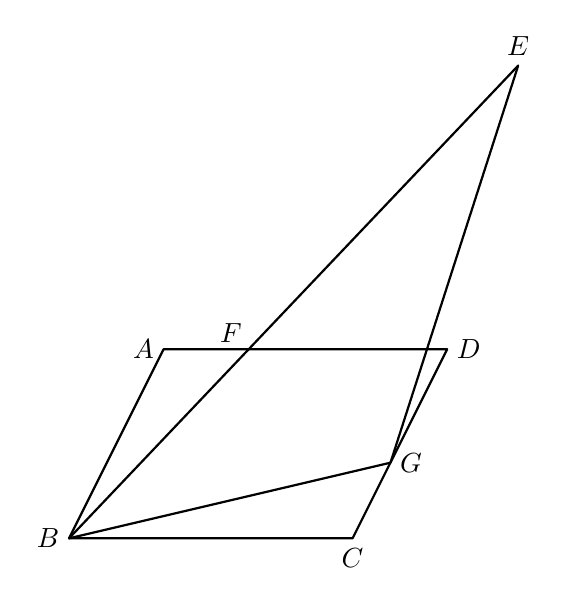
\begin{tikzpicture}[>=stealth, scale=1.2, line join=round, line cap=round]
    % 1. 定义平行四边形 ABCD 的顶点坐标
    \coordinate (B) at (0,0);
    \coordinate (C) at (3,0);
    \coordinate (A) at (1,2);
    % 利用向量加法计算 D 点：D = A + (C - B)
    \coordinate (D) at ($(A)+(C)-(B)$);

    % 2. 定义 F 点（在 AD 边上）和 G 点（在 CD 边上）
    % 可以通过 pos 参数调整比例以符合原图视觉
    \coordinate (F) at ($(A)!0.3!(D)$);
    \coordinate (G) at ($(C)!0.4!(D)$);

    % 3. 延长 BF 到点 E
    % 用比例因子 2.5 将 BF 延长至 E
    \coordinate (E) at ($(B)!2.5!(F)$);

    % 4. 绘制图形轮廓
    % 绘制平行四边形
    \draw[thick] (A) -- (B) -- (C) -- (D) -- cycle;

    % 绘制连接连线
    \draw[thick] (B) -- (E); % 穿过 F 的射线/线段
    \draw[thick] (E) -- (G); % 连接顶点 E 与边上点 G
    \draw[thick] (B) -- (G); % 连接 B 和 G

    % 5. 标注顶点标签
    % 根据原图位置调整标签方位 (above, below, left, right)
    \node[left] at (A) {$A$};
    \node[left] at (B) {$B$};
    \node[below] at (C) {$C$};
    \node[right] at (D) {$D$};
    \node[above] at (E) {$E$};
    \node[above left=-1pt] at (F) {$F$};
    \node[right] at (G) {$G$};

\end{tikzpicture}

\end{document}